\documentclass[openany]{book}
\usepackage{graphicx} % Required for inserting images
\usepackage{amsmath}
\usepackage{enumerate}
\usepackage{enumitem}
\usepackage{epigraph}
\usepackage{lipsum}
% \usepackage{titlepages}
\usepackage{tikz}
\usepackage[a4paper, total={6in, 8in}]{geometry}

\usepackage{lipsum}
\usepackage[Glenn]{fncychap}
\renewcommand{\chaptername}{UNIT}
\ChNameUpperCase
\ChNumVar{\fontsize{40}{42}\usefont{OT1}{ptm}{m}{n}\selectfont}
\ChTitleVar{\Large\sc}

\title{Sociology 141 - Social Movements \& Political Action}
\author{Alejandro Sanchez Ocegueda}
\date{Last updated: \today}

\newcommand{\st}{$^{\text{st}}$}
\newcommand{\nd}{$^{\text{nd}}$}
\newcommand{\rd}{$^{\text{rd}}$}
\renewcommand{\th}{$^{\text{th}}$}

\renewcommand\epigraphflush{flushright}
\renewcommand\epigraphsize{\normalsize}
\setlength\epigraphwidth{0.7\textwidth}

\definecolor{titlepagecolor}{cmyk}{1,.60,0,.40}

\DeclareFixedFont{\titlefont}{T1}{ppl}{b}{it}{0.5in}

\makeatletter                       
\def\printauthor{%                  
    {\large \@author}}              
\makeatother
\author{%
    Alejandro Sanchez Ocegueda \\
    % Updated \today \\
    Spring 2025 \\
    \texttt{alexso@berkeley.edu}\vspace{20pt}
    % Department name \\
    }

% The following code is borrowed from: https://tex.stackexchange.com/a/86310/10898

\newcommand\titlepagedecoration{%
\begin{tikzpicture}[remember picture,overlay,shorten >= -10pt]

\coordinate (aux1) at ([yshift=-15pt]current page.north east);
\coordinate (aux2) at ([yshift=-410pt]current page.north east);
\coordinate (aux3) at ([xshift=-4.5cm]current page.north east);
\coordinate (aux4) at ([yshift=-150pt]current page.north east);

\begin{scope}[titlepagecolor!40,line width=12pt,rounded corners=12pt]
\draw
  (aux1) -- coordinate (a)
  ++(225:5) --
  ++(-45:5.1) coordinate (b);
\draw[shorten <= -10pt]
  (aux3) --
  (a) --
  (aux1);
\draw[opacity=0.6,titlepagecolor,shorten <= -10pt]
  (b) --
  ++(225:2.2) --
  ++(-45:2.2);
\end{scope}
\draw[titlepagecolor,line width=8pt,rounded corners=8pt,shorten <= -10pt]
  (aux4) --
  ++(225:0.8) --
  ++(-45:0.8);
\begin{scope}[titlepagecolor!70,line width=6pt,rounded corners=8pt]
\draw[shorten <= -10pt]
  (aux2) --
  ++(225:3) coordinate[pos=0.45] (c) --
  ++(-45:3.1);
\draw
  (aux2) --
  (c) --
  ++(135:2.5) --
  ++(45:2.5) --
  ++(-45:2.5) coordinate[pos=0.3] (d);   
\draw 
  (d) -- +(45:1);
\end{scope}
\end{tikzpicture}%
}

\begin{document}
\begin{titlepage}
\noindent
\titlefont Social Movements \par
\epigraph{Pure mathematics is on the whole distinctly more useful than applied. For what is useful above all is technique, and mathematical technique is taught mainly through pure mathematics.}%
{\textit{London 1941}\\ \textsc{G. H. Hardy}}
\null\vfill
\vspace*{1cm}
\noindent
\hfill
\begin{minipage}{0.35\linewidth}
    \begin{flushright}
        \printauthor
    \end{flushright}
\end{minipage}
%
\begin{minipage}{0.02\linewidth}
    \rule{1pt}{125pt}
\end{minipage}
\titlepagedecoration
\end{titlepage}

\tableofcontents

\chapter{Social Movements \& Sociology}
% Date: January 21st

\counterwithout{section}{chapter}
\noindent \textbf{Lecture 1 --- January 21\st}

\section{Approaches to Social Movements}
In this first section, we first give a brief overview of the different approaches to studying social movements and political action.


\subsection{The Pluralist Approach}
% TODO
The argument of the pluralist was that the US was good because the system included a plurality of interests (hence the name).
The idea was that even if there were imbalances and inequalities, the political power was widely distributed between competing groups;
that is, no one group completely controls the system.


\subsection{The Classical Approach}

The classical approach refers to the way scholars and sociologists studied social movements before the 1970s.

Fun fact: the course is titled \textit{Social Movements \& Political Action}.
In the classical approach.

Aside: Political Action.
Before, the study of social movements was relegated to social psychology, mostly because it was viewed as an irrational action.
It was categorized as a form of ``deviance.''
They were viewed as ``pathological'' or ``irrational''.

% \section{Political Sociology}

Political Science and Political Sociology studied Institutional Politics, whereas Social Psychology studied Insurgent Politics

\textbf{Institutional Politics:} Politicis within formal institutional channels.
For instance, electoral processes.
During the classical times, only institutional politics were viewed as ``real'' politics. 
Other forms of politics (often known as insurgent politics) were viewed as ``not real'' politics.

\noindent \textbf{Insurgent Politics:} Collective behavior (?)

Pluralist approach $\Rightarrow$ Classical approach

The classical approach is based on the pluralist approach to politics.


The underlying assumption is that the competition between the different political groups would balance out the disparity among them.
This, in theory, ensured that the political system was
\begin{enumerate}
    \item \textbf{Open:} no group monopolizes power to block other groups.
    \item \textbf{Responsive:} the need for coalitions necessitates responding to the demands of other groups.
\end{enumerate}

This was the dominant theory during the 1960s.

C Wright Mills refers to this as ``Elite Theory.''

\subsection{The Elite Theory Approach}
This is a new approach first proposed by C. Wright Mills, and it centers around the concept of the ``elite.''

\noindent \textbf{Elite:} those who hold power in a society.
The idea transitioned from the Elite Theory to the Resource Mobilization approach.

The postulates of Elite Theory are as follows:
\begin{enumerate}
    \item The system is controlled by the elite
    \item Most groups are politically excluded
\end{enumerate}

\subsection{The Resource Mobilization Approach}
This new approach is based on the Elite Theory approach to politics. 

\subsection{Why care about all these approaches?}
Today, all of this falls under the ``Political Action'' umbrella term.
Furthermore, the classical approach has been completely rejected.
But why is it worth our time?
In part, it is important to know about these things because understanding these old approaches gives you a sense of what newer scholars are arguing against.
Most importantly, it is important to understand how social movements were often cast to the wayside and treated as irrational and deviant.
These ideas and assumptions, antiquated and refuted as they are, continue to shape the way people think and approach social movements to this very day.


\section{Social Movements}
There are several questions we will address throughout this course

\begin{enumerate}
    \item Emergence: under what conditions do mass social movements to emerge?
    How can we learn to recognize those conditions so that we can fully exploit them when they show up?
    \item Objectives:
    What have social movements sought to achieve?
    \item Strategies/Tactics: What different kinds of tactics have been used to attain those objectives? 
    Which strategies and tactics have been effective?
    What factors influence the efficacy?
    \item Organization:
    How have different movements organized themselves?
    What different forms of organization have they adopted?
    \item Challenges:
    What kinds of challenges have different movements faced?
    What different state oppression have movements been challenged with?
    How have different movements responded or adapted to those challenges?
    \item Impact:
    How can we fully assess the impacts of movements?
    What have been their intended impacts?
    What have been the unintended impacts or reverberations of social movements?
\end{enumerate}


% \counterwithout{section}{chapter}

\vspace{3mm}
\noindent \textbf{Lecture 2 --- January 23\rd}

\section{The Structuring of Protest}
At the heart of sociology, there is an ongoing debate between the importance of agency and structure.
Agency is defined to be the capacity of human beings to act independently.
Structuralism is a branch of sociological belief that emphasizes that agency is shaped and constrained by the structures of society.
One can think of this debate as a continuum, where all sociologists lay in some point, giving more or less important to agency and structure.

\begin{center}
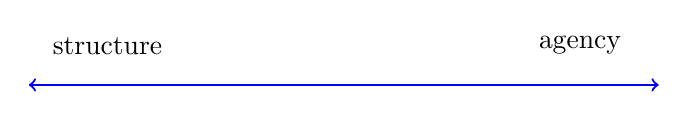
\begin{tikzpicture}
    \draw[thick, <->, blue] (0,0)  -- (8, 0);
    \draw (1, 0.5) node{structure};
    \draw (7, 0.5) node{agency};
    \draw[.] (5,0);
\end{tikzpicture}
\end{center}

Q: Is agency required for structure to arise?

Piven and Cloward make a structuralist argument regarding social movements.
More specifically, they argue that the structure of society influences when movements can arise, what shape the movements will take, and how effective they will be.

\begin{center}
\textit{``In seeking to do what wasn't possible, we failed to do what was... (p. TODO)''}
\end{center}

Notably, Piven \& Cloward offer their own ideas of what a social movement is.
In other words, what should count as a social movement (pp. 3-4).
The two main criteria that they propose are that there should be (a) a transformation of consciousness, and (b) a transformation of behavior.

\subsection{Transformation of Consciousness}
We summarize the criteria that Piven \& Cloward give for a transformation of consciousness below:
\begin{enumerate}
    \item \textit{The system loses legitimacy:}
    In other words, people view the structure of society as unjust and wrong.
    This should not be surprising.
    In fact, most people, at most points in time, believe that society is unjust and wrong (at least to some extent).
    However, this is still an important and necessary condition for a social movement to arise (at least according to Piven \& Cloward).
    \item \textit{Alternatives seem possible:}
    Unlike most of the time, people think that there indeed does exist another way of living.
    \item \textit{Sense of efficacy:}
    Finally, the people come to believe that not only is the system wrong and that there exists a viable alternative, but that this alternative is indeed something that is attainable.
\end{enumerate}
There is a sort of implicit precedence between these three criteria.
Before people think that they can change their living situation to something better, they must have an idea of what the alternative is in mind, and before people conceive that alternative, it is necessary that they see something that is wrong and requires change within their current conditions.

\subsection{Transformation of Behavior}

\begin{enumerate}
    \item \textit{Masses of people become defiant:}
    By this, we mean that people begin to break the rules and norms established in society.
    These can be formal rules (such as the law), or cultural rules.
    Not all movements break the law, but all movements break some form of social norm.
    \item \textit{Defiance is acted out collectively:}
    It is not only necessary that rules and norms are broken by the people, but that people engaging in this disobedience also believe that they are acting as part of a larger group or movement.
\end{enumerate}
Succinctly, we can say 
\begin{center}
\textit{``A protest movement is collective defiance fueled by a transformation of consciousness.''}  
\end{center}


\section{Emergence of Protest Movements}
Now that we have discussed \textit{what} social movements are, a natural question to ask is \textit{when} social movements \textbf{emerge}.
Piven \& Cloward give a characterization for the conditions necessary to spark a social movement.

\begin{enumerate}
    \item \textit{Massive social or economic changes:}
    There must be a rapid and drastic change in the living conditions of a large group of people.
    This can be a massive migration, industrialization, depression, or any other number of such large-scale events.
    \item \textit{Institutional breakdown:}
    The aforementioned massive social/economic changes begin to strain the institutions.
    For example, an economic force like a depression can put a lot of strain on a number of institutions.
    This, importantly, disrupts the routines of people's daily lives.
    \item \textit{Transformation of consciousness:} 
    These two conditions put together, cause a profound \textbf{social dislocation}.
    Informally, people's lives are thrown out of whack.
    This is often sufficient to cause a transformation of consciousness, of the kind we had defined and talked about at length previously.
    \item \textit{Division \& competition among elites:}
    The vested interest of the ruling class is in preserving the status quo.
    Mostly, they are unified in their interest in maintaining the status quo.
    Nonetheless, periods of massive economic change and social upheaval can create fissures among the elite class.
    This can cause dissonance and delegitimize their authority.

\end{enumerate}
Once again, Piven \& Cloward provide us with a fancy quote to characterize these criteria:
\begin{center}
\textit{``The social arrangements that are ordinarily perceived as just and immutable must come to be perceived as unjust and mutable (p. TODO).''}
\end{center}


% \chapter{The Power of Disruption: The Movement of the Unemployed}


% \newpage
% \chapter{Strategic \& Tactical Dynamics: The Civil Rights Movement}

% \chapter{Unintended Impacts: Countermovements \& Electoral Reverberations}

% \chapter{``Free Speech'': UC Berkeley from the FSM to the Palestine Solidarity Movement}

% \chapter{``Black Power'' and its Progenies: The Black Panther Party \& the New Left}

% \chapter{The Dynamics of Repression}

% \chapter{The Stonewall Riots \& the Gay and Trans Liberation Movements}

% \chapter{Occupy \& the ``Violence'' of Resistance}

% \chapter{The Dialectic of Repression \& Resistance: ``Black Power'' to ``Black Lives Matter''}

% \chapter{Indigenous Resistance: From ``Red Power'' to Standing Rock}

% \chapter{The Movement for Black Lives}




\end{document}